\documentclass{article}
\usepackage{setspace}
\usepackage{listings}
\usepackage{color}
\usepackage{amsmath}
\usepackage{amssymb}
\usepackage{amsthm}
\usepackage{graphicx} 
\usepackage{float} 
\usepackage{fancyhdr}                                
\usepackage{lastpage}                                           
\usepackage{layout}   
\usepackage{subfigure} 
\definecolor{codegreen}{rgb}{0,0.6,0}
\definecolor{codegray}{rgb}{0.5,0.5,0.5}
\definecolor{codepurple}{rgb}{0.58,0,0.82}
\definecolor{backcolour}{rgb}{0.95,0.95,0.92}

\lstdefinestyle{mystyle}{
    backgroundcolor=\color{backcolour},   
    commentstyle=\color{codegreen},
    keywordstyle=\color{magenta},
    numberstyle=\tiny\color{codegray},
    stringstyle=\color{codepurple},
    basicstyle=\footnotesize,
    breakatwhitespace=false,         
    breaklines=true,                 
    captionpos=b,                    
    keepspaces=true,                 
    numbers=left,                    
    numbersep=5pt,                  
    showspaces=false,                
    showstringspaces=false,
    showtabs=false,                  
    tabsize=2
}
\pagestyle{fancy}  
\lhead{ZHANG HUAKANG}
\chead{Assignment 4} 
\rhead{DB92760} 
\renewcommand{\baselinestretch}{1.05}
\title{Assignment 4 of CISC 2002}
\author{ZHANG Huakang/DB92760}

\begin{document}
    \maketitle
    \section{}
        \subsection{}
        \lstinputlisting[language=Matlab,style=mystyle,caption=Code ]{code/Assignment_4_1_1.m}
        \lstinputlisting[language=Matlab,style=mystyle,caption=Output ]{code/Assignment_4_1_1_output}
        We can get the function
        $$f(x)=0.4143 x+1.6000$$
    \subsection{}
        \begin{equation*}
            \begin{split}
                f(14)=&0.4143\times 14+1.600\\
                    =&7.4002\\
            \end{split}
        \end{equation*}
    \subsection{}
        \begin{figure}[H] 
            \centering 
            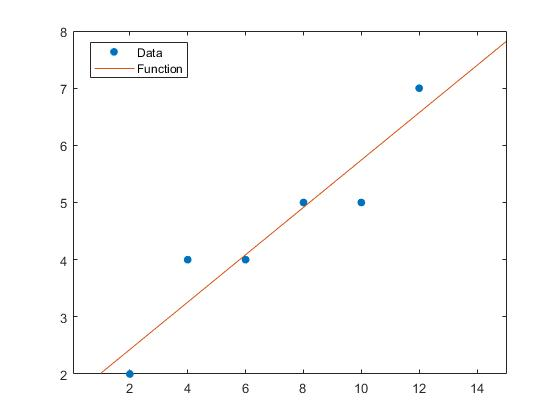
\includegraphics[width=0.9\textwidth]{img/Assignement_4_1_1.jpg}
            \caption{Figure} 
        \end{figure}
    \section{}
        \subsection{}
            \begin{equation*}
                \begin{split}
                    y=&Ce^{Ax}\\
                    \log y=& \log C + Ax\\
                \end{split}
            \end{equation*}
            \lstinputlisting[language=Matlab,style=mystyle,caption=Code ]{code/Assignment_4_2_1.m}
            \lstinputlisting[language=Matlab,style=mystyle,caption=Output ]{code/Assignment_4_2_1_output}
            We can get
            \begin{equation*}
                \begin{split}
                    A=&0.6288\\
                    C=&e^\beta\\
                        =&1.0849 
                \end{split}
            \end{equation*}
        \subsection{}
            \begin{figure}[H] 
                \centering 
                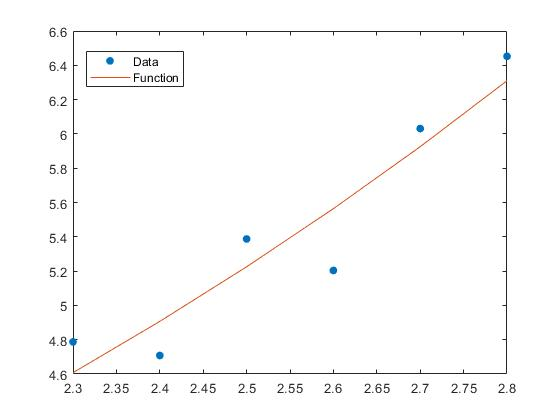
\includegraphics[width=0.9\textwidth]{img/Assignement_4_2_1.jpg}
                \caption{Figure} 
            \end{figure}
    \newpage
    \section{}
        \subsection{}
        \lstinputlisting[language=Matlab,style=mystyle,caption=Code ]{code/Assignment_4_3_1.m}
        \lstinputlisting[language=Matlab,style=mystyle,caption=Output ]{code/Assignment_4_3_1_output}
        \begin{equation*}
            \begin{split}
                c=&1.0077\\
                y=&1.0077\sin(x)
            \end{split}
        \end{equation*}
    \subsection{}
        \begin{figure}[H] 
            \centering 
            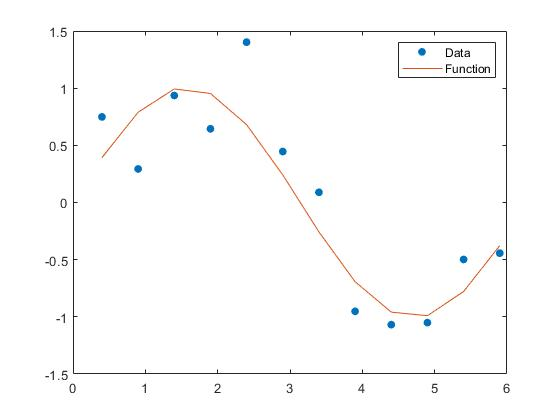
\includegraphics[width=0.9\textwidth]{img/Assignement_4_3_1.jpg}
            \caption{Figure} 
        \end{figure}
    \section{}
        \subsection{}
            \begin{figure}[H] 
                \centering 
                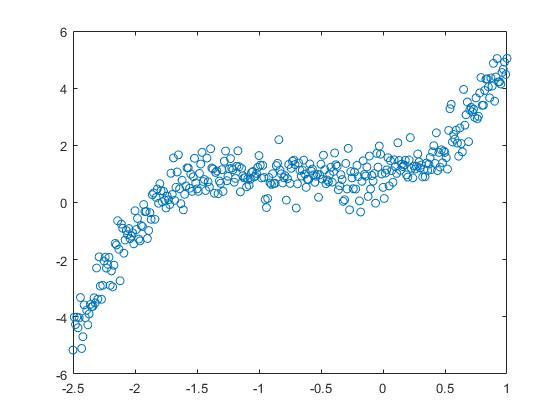
\includegraphics[width=0.9\textwidth]{img/Assignement_4_4_1.jpg}
                \caption{Figure} 
            \end{figure}
        \subsection{}
            \begin{equation*}
                \begin{split}
                    f_1(x)=&1\\
                    f_2(x)=&x\\
                    f_3(x)=&x^2\\
                    f_4(x)=&x^3\\
                \end{split}
            \end{equation*}
        \subsection{}
            \lstinputlisting[language=Matlab,style=mystyle,caption=Code ]{code/Assignment_4_4_1.m}
            \lstinputlisting[language=Matlab,style=mystyle,caption=Output ]{code/Assignment_4_4_1_output}
            $$y=0.9156+0.8796x+2.1602x^2+1.0880x^3$$
        \subsection{}
            \begin{figure}[H] 
                \centering 
                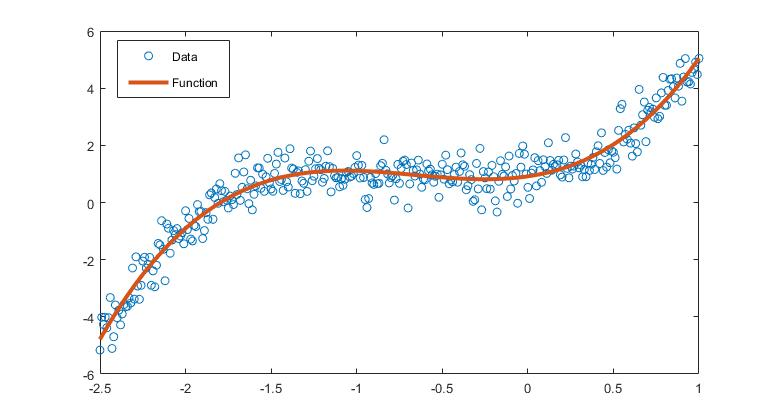
\includegraphics[width=1\textwidth]{img/Assignement_4_4_2.jpg}
                \caption{Figure} 
            \end{figure}
\end{document}